% Teaching Statement — standalone compilable version (locked Sept 2026).
% Output: Teaching_Statement_Sachdeva.pdf -> teaching/
% Requires evals_summary_figure.pdf alongside this file.
\documentclass[letter,11pt]{article}
\usepackage[margin=0.97in, headheight=60pt]{geometry} % Ensuring proper header space
\usepackage{parskip} % Adds space between paragraphs
\usepackage{enumitem} % For list customization
\usepackage{hyperref} % For hyperlinks
\usepackage{titlesec} % For section title formatting
\usepackage{fontawesome} % For icons (email, phone, etc.)
\usepackage{xcolor} % For color
\usepackage{fancyhdr} % For header and footer
\usepackage{array} % For better alignment control
\usepackage{tabularx} % To control column width
\usepackage[normalem]{ulem} % For underlining styles
\usepackage{calligra} % Calligra handwritten font package
\usepackage{xcolor} % Optional: for customizing font color
\usepackage{mathrsfs}
\usepackage{pdfpages}

% --- Added for the teaching documents (figures, captions, tables) ---
\usepackage{graphicx}
\usepackage{caption}
\usepackage{booktabs}
% --------------------------------------------------------------------

\usepackage{multicol} % For multiple columns
\setlength{\columnsep}{0.1cm} % Adjusts the spacing between columns
\usepackage{ragged2e}

% Define darkslategray using RGB
\definecolor{darkslategray}{RGB}{47, 79, 79} 
\definecolor{airforceblue}{rgb}{0.36, 0.54, 0.66}

% Font for a more artsy and modern vibe
\usepackage{libertine} % Professional but unique font family
\renewcommand{\familydefault}{\sfdefault} % Switch to sans-serif for headers

% Header formatting with color and layout adjustments
\fancypagestyle{firstpage}{ % Define a custom style for the first page
  \fancyhf{} % Clear all header and footer fields
  \fancyhead[L]{\textbf{\LARGE Gagandeep Sachdeva}\\Post-Doctoral Fellow, JPAL South Asia}
  \fancyhead[R]{\\
  
      \href{mailto:gsachdeva@povertyactionlab.org}{\faEnvelope\ gsachdeva@povertyactionlab.org} \\
      \faPhone\ +1 (831)-295-3570 \\
      %\href{https://scholar.google.com/citations?user=hwENZWUAAAAJ&hl=en}{\faGlobe\ Google Scholar}\\
      \href{https://gagandeep-sachdeva.com/}{\faGlobe\ Personal Website}
  }
  \fancyfoot[C]{\thepage} % Page number centered in footer
}
\pagestyle{plain} % Plain page style for subsequent pages (no header, only page number in footer)


% Set hyperlink color to blue
% Define a light background color for links
\definecolor{highlightbg}{RGB}{230, 230, 230}
\definecolor{darkgrayishblue}{RGB}{60, 70, 85} % More gray than blue but distinguishable

% Set up hyperlinks with custom styling
\hypersetup{
    colorlinks=true, % Enable colored links
    linkcolor=darkslategray, % Use dark grayish blue for links
    urlcolor=darkslategray,  % URL color using dark grayish blue
    citecolor=darkslategray, % Citation links color
    filecolor=darkslategray  % File links color
}

% Define custom hyperlink formatting: bold or slight emphasis with the new color
\renewcommand\UrlFont{\color{darkgrayishblue}\itshape} % Italicized dark grayish blue links
% Section title formatting with color and underline
\titleformat{\section}
{\color{darkslategray}\large\bfseries}{}{0em}{}[\titlerule] % Use defined darkslategray

% Custom bullets for lists
\renewcommand{\labelitemi}{\scriptsize\textcolor{darkslategray}{$\blacksquare$}} % Dark slate gray-colored square bullets

% Set nested list indentation levels
\setlist[itemize,1]{left=0pt, label={\scriptsize\textcolor{darkslategray}{$\blacksquare$}}}
\setlist[itemize,2]{left=20pt, label={\scriptsize\textcolor{darkslategray}{$\bullet$}}} % Nested level 2
\setlist[itemize,3]{left=40pt, label={\scriptsize\textcolor{darkslategray}{$-$}}}       % Nested level 3

% Adjust list indentation and paragraph spacing
\setlist[itemize]{leftmargin=0}
\setlist[enumerate]{leftmargin=0}
\setlength{\parskip}{0.5em}



% Command to right-align dates
\newcommand{\dateright}[1]{\hfill{\small #1}}

\begin{document}

\newcommand{\studentquote}[1]{\begin{quote}\itshape ``#1''\end{quote}}

\thispagestyle{firstpage}
\begin{center}
    \textbf{\large{Teaching Statement}}
\end{center}

A good education in economics encourages students to think critically, charitably, and collaboratively about the world around them. Doing that takes effort and persistence -- non-cognitive dimensions of learning that my research explores -- and my teaching is designed to make both effort and persistence an everyday part of learning. In practice this means (a) material broken into steps students can execute before they are asked to combine them, (b) sections wherein every student is expected to contribute, and (c) help-seeking that is encouraged and expected. I was able to develop and practice this approach as both an instructor-of-record and a teaching assitant across sixteen courses at UC Santa Cruz, including lower-division principles courses, intermediate and advanced microeconomics, and graduate-level courses in applied microeconomics and econometrics.

For me, a typical lecture or section involves students working with material in ways that effort is continuously rewarded, usually by breaking down a day's learning objectives into small, bite-sized pieces. For instance, when I teach utility maximization, each practice problem is scaffolded into standalone tasks: writing the budget constraint, finding its slope, computing marginal utilities, setting up the Lagrangian. I design graded problems that sequentially remove this scaffolding, so students assemble a solution they have already built in parts. I also write practice problems that mirror the ones that students would be assessed on; in my most recent course, three students independently named these as the practice that helped them most. Section design and assessment design are two ends of the same alignment: both should follow from the learning outcomes of the course. As instructor of record for Intermediate Microeconomics, I set both -- learning goals stated at the outset, with problem sets and examinations written to reflect proficiency in those learning goals.\footnote{The course was scheduled in person and moved to asynchronous online delivery two weeks before the term; I redesigned the materials and assessment sequence for that format. $n = 11$ respondents.} All nine respondents to the item said the problem sets prepared them for the examinations, and nine out of eleven respondents reported that they understood the course's learning outcomes from the beginning. Two courses I have designed -- Principles of Economics and Current Debates in Economics -- carry the same alignment through a full grading scheme: every assignment supports a stated learning outcome, and concept-mastery quizzes stay open for a week with unlimited attempts, so the grade rewards persistence rather than a first attempt.\footnote{Sample syllabi for both courses are available on my teaching page.} Across the thirteen courses with comparable evaluations, a weighted 95 percent of respondents say I explained concepts in ways that supported their learning (Appendix Figure~1).\footnote{Percentages exclude respondents answering ``unable to comment.'' Weighted averages weight each course-item cell by the number of respondents and by recency. Response rates to teaching-assistant items vary across courses and are reported with Appendix Figure~1. The full set of evaluations is available at \href{https://gagandeep-sachdeva.com/teaching.html}{my teaching page}.
}

\studentquote{He was able to break down concepts in ways to where I actually understood course material instead of just going through the motions of solving problems using set equations.}

Sections are built so that every student is encouraged and expected to contribute -- I call on students in turn to supply the next step of a problem, and when a step is wrong, we work out why before moving on. In graduate econometrics, the same expectation runs through code: rather than distributing finished Stata programs, I build them with the class, with students proposing each step before we implement it. In that course, sections were optional; every survey respondent attended at least three of the ten weekly meetings, and 88 percent attended eight or more.\footnote{Seventeen of nineteen enrolled students responded to the survey. Across my five most recent courses pooled, 77 percent of respondents attended three or more sections where attendance was optional.}

\studentquote{Gagandeep Sachdeva also made us pass around a talking stick to answer what step/method of the question we do. This made me stay on my toes and be engaged with the material even if we would say the wrong thing Gagandeep would help guide us and learn our mistakes in a way that didn't make us scared to make mistakes.}
\studentquote{I appreciated how interactive Gagandeep made sections. It was helpful that he encouraged every student interact instead of letting one or two students answer everything. Being somewhat put on the spot, or expected to engage helped me learn and engage with the material.}

I make asking for help routine from the first week of a course. Questions are treated as expected: class time includes regular low-stakes opportunities to ask them, and office hours are informal. In the courses I have designed, the same expectation is written into policy: every student receives dropped attendances and no-questions-asked extensions automatically, so a difficult week never requires asking for an exception. A weighted 96 percent of respondents across all courses say I made them feel as though they could succeed in the class.

\studentquote{I appreciate your approachability, I am typically pretty shy but I never felt hesitant to ask questions during or outside of section.}

My teaching work extends past my own sections. As a Graduate Pedagogy Fellow for UCSC's economics department, I created its workshop series for graduate teaching assistants -- four sessions on defining learning goals for a section, building active-learning activities for introductory and intermediate courses, and giving effective feedback -- and led it for three years. In a separate quarter-long workshop, TAs met with me weekly to design their upcoming sections together. In feedback collected after the first round of the series, participants who had attended the department's earlier trainings noted the difference, and several described practices they had already carried into their own sections.\footnote{$n = 8$ participants; feedback was collected after the Fall 2023 round.} As a peer mentor on the Teaching and Learning Center's Summer GSI Support Team, I reviewed syllabi and assessment plans with first-time instructors across STEM fields.

\studentquote{This training had a strong emphasis on pedagogy and good teaching practices which was completely absent from previous trainings. This was a glaring gap, as many of the entering graduate students are teaching for the very first time.}
\studentquote{As a fairly experienced TA, I was stuck in a rut \dots\ these workshops gave me ideas [for] how to prepare for sections differently and make it more interesting. For example, while teaching my students about production costs, I conducted an exercise wherein I asked the students to come up with their own business ideas and frame a cost table \dots\ These and other active learning exercises have helped me to engage with my students more and it seems to be helping them too.}

\clearpage
\begin{figure}[htbp!]
\captionsetup{labelformat=empty}
    \caption*{Appendix Figure 1: Student evaluations of teaching, 2020--2026. Weighted shares of respondents answering ``frequently'' or ``very frequently'' are between 90 and 97 percent on all ten items.}
    \centering
    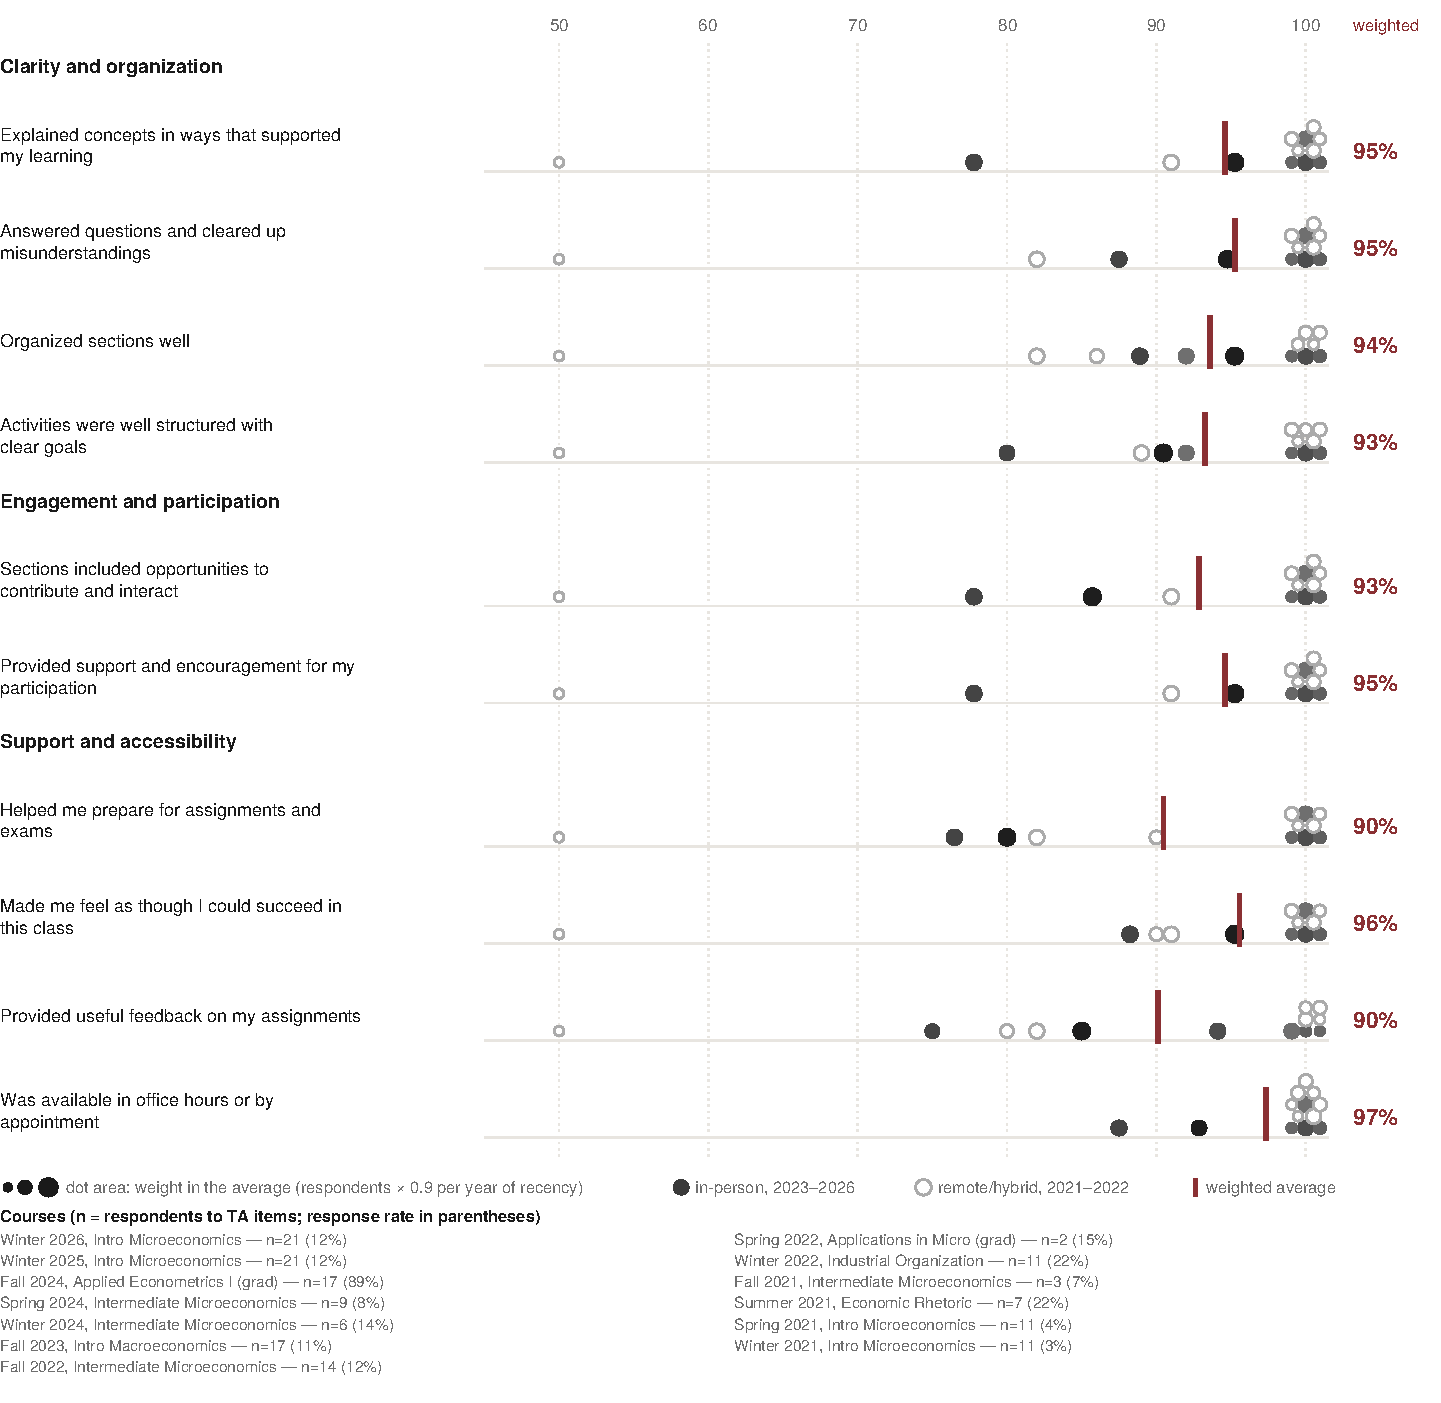
\includegraphics[width=\linewidth]{evals_summary_figure.pdf}
    \par\vspace{4pt}
    {\footnotesize\raggedright Notes: Each dot depicts the share of respondents who responded with ``frequently" or ``very frequently" on a given evaluation item for a given course. The size of the dot depicts the weight of the course in the overall average -- based on the number of respondents and recency. Filled dots are in-person courses, Fall 2023--Winter 2026; open circles are remote- and hybrid-era courses, 2021--2022. Maroon bars mark weighted averages.\par}
\end{figure}

\end{document}
